\section{Diseño}
Todos los amplificadores operacionales utilizados en las etapas a continuación corresponden a LM358, todos los transistores NPN corresponden a 2N3904, y todos los diodos corresponden a 1N4001.
\subsection{Circuito oscilador en cuadratura}
Se escogió utilizar el oscilador en cuadratura original que se muestra en la \figref{cuadraTopologies}.
De forma similar a como fue realizado en el experimento \#2 del curso, este circuito presenta realimentación positiva, a partir la cual se busca satisfacer el criterio de Barkenhausen para que el circuito genere una oscilación mantenida. 
Sean $R_1$, $C_1$, $R_2$, $C_2$, y $R_3$, $C_3$ los pares de componentes RC en los lazos de retroalimentación negativa de los amplificadores operacionales que se muestran en la \figref{cuadraTopologies}, así como el circuito RC que realimenta una etapa de amplificación con otra. 
Se debe satisfacer la condición \eqref{condicionOscilacion} para que se genere una oscilación mantenida en el circuito \cite{franco2015opamps}, asumiendo que la salida del circuito es la salida de la primera etapa de amplificación del circuito (COS).
\begin{equation}
    R_1 C_1 = R_2 C_2 = R_3 C_3\label{condicionOscilacion}
\end{equation}
La frecuencia de oscilación del circuito viene dada por la ecuación \eqref{freqOscilacion}.
Esta se escoje que tenga un valor de \SI{260}{Hz}.
\begin{equation}
    f = \frac{1}{2\pi RC}\label{freqOscilacion}
\end{equation}
Donde $RC$ es la multiplicación de los valores de alguno de los pares RC del circuito, los cuales todos deben de tener el mismo valor, idealmente.
Adicionalmente, debido a que el circuito tiene una segunda etapa de amplificación que consiste de un amplificador integrador, se obtiene una salida adicional correspondiente a la integral de la primera salida de tensión. 
Debido a que la primera salida corresponde a una señal coseno, la segunda salida corresponderá a una señal seno.
Gracias a esto se obtienen dos señales sinusoidales desfasadas $\pi/2$ una con respecto a la otra.

Se simuló este oscilador en LTSpice, dando una tensión inicial distinta de \SI{0}{V} a los capacitores en el circuito, lo cual permite que arranque la oscilación mantenida en un ambiente controlado como lo es el software de simulación.
El circuito simulado se muestra en la \figref{cuadraturaCir}, mientras que ambas salidas del circuito se muestran en la \figref{cuadraturaSim}.

\newpage
\begin{figure}[H]
    \centering
    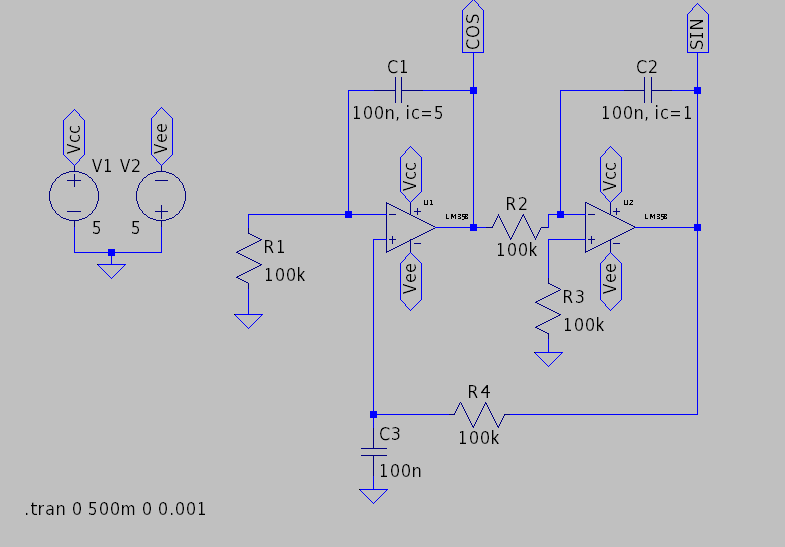
\includegraphics[width=0.75\linewidth]{figs/diseño/1osciladorCir.png}
    \caption{Oscilador en cuadratura simulado en LTSpice}
    \label{cuadraturaCir}
\end{figure}

\begin{figure}[H]
    \centering
    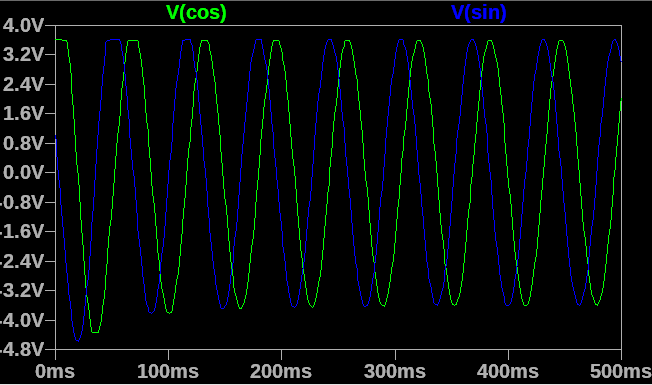
\includegraphics[width=0.75\linewidth]{figs/diseño/1osciladorSim.png}
    \caption{Salidas del oscilador en cuadratura simulado en LTSpice}
    \label{cuadraturaSim}
\end{figure}

Como se puede observar en la \figref{cuadraturaSim}, ambas señales están desfasadas por $\pi/2$, siendo este el resultado esperado de la simulación.
Tomando en cuenta la experiencia adquirida en el segundo laboratorio del curso con circuitos osciladores, se escoge que las resistencias $R_1$, $R_2$, y $R_3$ se implementen por medio de trimmers de \SI{250}{\kohm} cada una, $T_1$, $T_2$, y $T_3$, con el propósito de ajustar lo mejor posible la condición de oscilación \eqref{condicionOscilacion}, ya que puede ser afectada por múltiples aspectos reales del circuito, como por ejemplo, la tolerancia en las capacitancias, la cual suele ser alta. 

\subsection{Circuitos desfasadores de 360° y comparadores ajustables}
Estos circuitos no fueron modificados con respecto al diseño original \cite{pong}.
Se simuló solo uno de ellos, debido a que ambos circuitos son equivalentes uno con respecto al otro, siendo la única diferencia la fase de la entrada sinusoidal aplicada. 
Debido a que no se pudo encontrar el modelo de un potenciómetro en LTSpice, se simularon por medio de resistencias individuales.
Las resistencias variables implementadas por medio del potenciómetro de doble gang fueron ajustadas a \SI{1}{\kohm} para poder observar un desfase en la salida del circuito desfasador con respecto a la entrada.
Adicionalmente, se ajustó el otro potenciómetro a su valor central para que se genere una señal cuadrada de aproximadamente el 50\% del ciclo del trabajo en la salida del comparador.
El circuito simulado se muestra en la \figref{desfasadorCir}, mientras que la señal de entrada, señal desfasada, y señal desfasada cuadrada se muestran en la \figref{desfasadorSim}.

\begin{figure}[H]
    \centering
    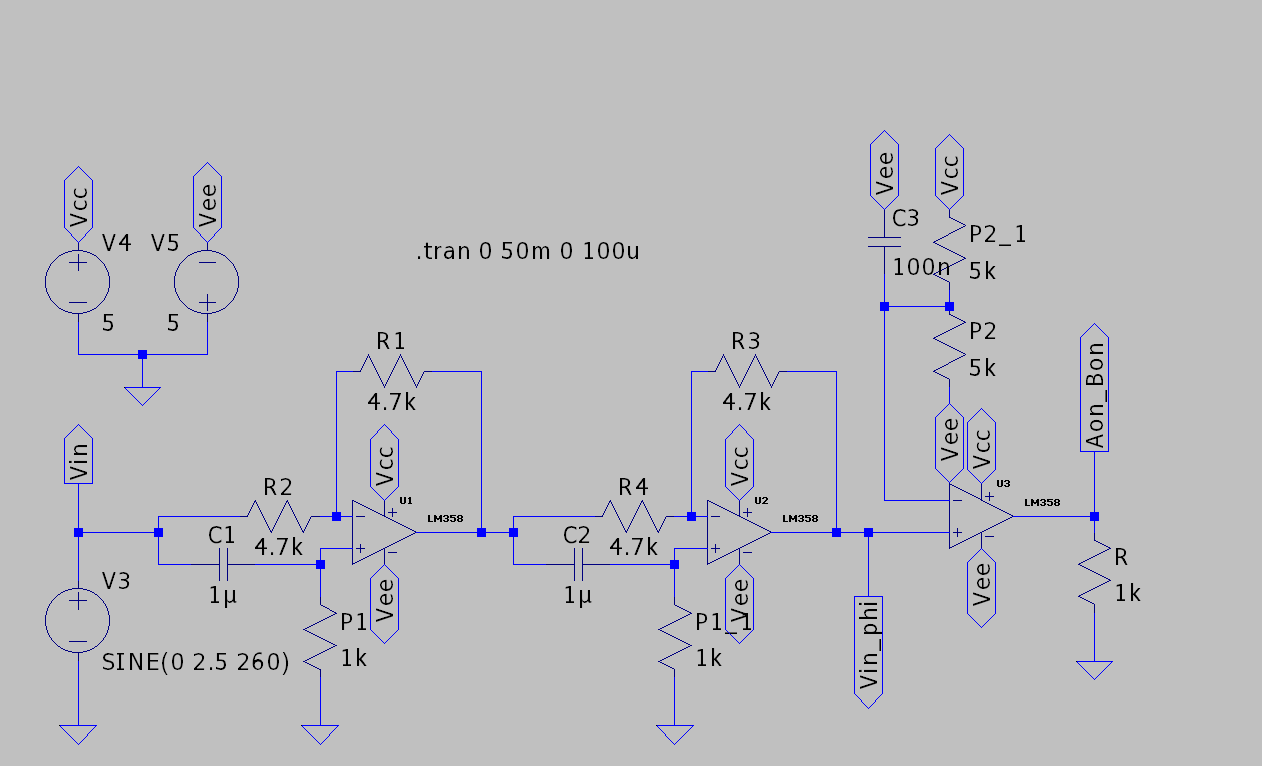
\includegraphics[width=0.65\linewidth]{figs/diseño/2desfasadorCir.png}
    \caption{Circuito desfasador de 360° y comparador ajustable simulado en LTSpice}
    \label{desfasadorCir}
\end{figure}

\begin{figure}[H]
    \centering
    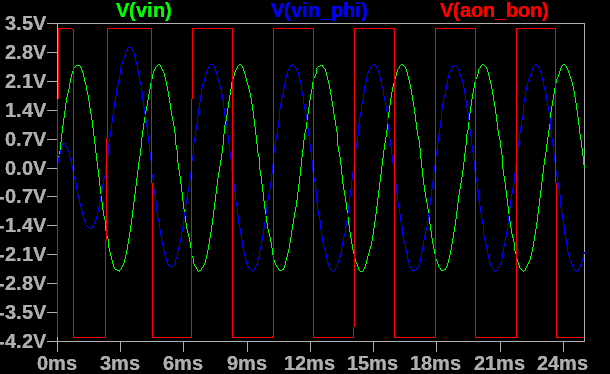
\includegraphics[width=0.65\linewidth]{figs/diseño/2desfasadorSim.png}
    \caption{Entrada, señal intermedia, y salida del circuito desfasador de 360° y comparador ajustable simulado en LTSpice}
    \label{desfasadorSim}
\end{figure}

Como se puede observar en la \figref{desfasadorSim}, el comportamiento de las señales del circuito es el esperado.
Un detalle importante que se debe tomar en cuenta en la forma que este circuito desfasa la señal de entrada es que se realiza de forma lineal debido a la función $\tan^{-1}$ que aparece al obtener la respuesta en frecuencia de cada desfasador de 180°, por lo que el movimiento de las paletas no será simétrico con respecto a la posición de las paletas en la pantalla en algún momento.

\subsection{Circuito con comparador y flip flop}
Se simuló este circuito en LTSpice, el cual se muestra en la \figref{clkCir}.
Las señales de entrada y salida del circuito se muestran en la \figref{clkSim}.

\begin{figure}[H]
    \centering
    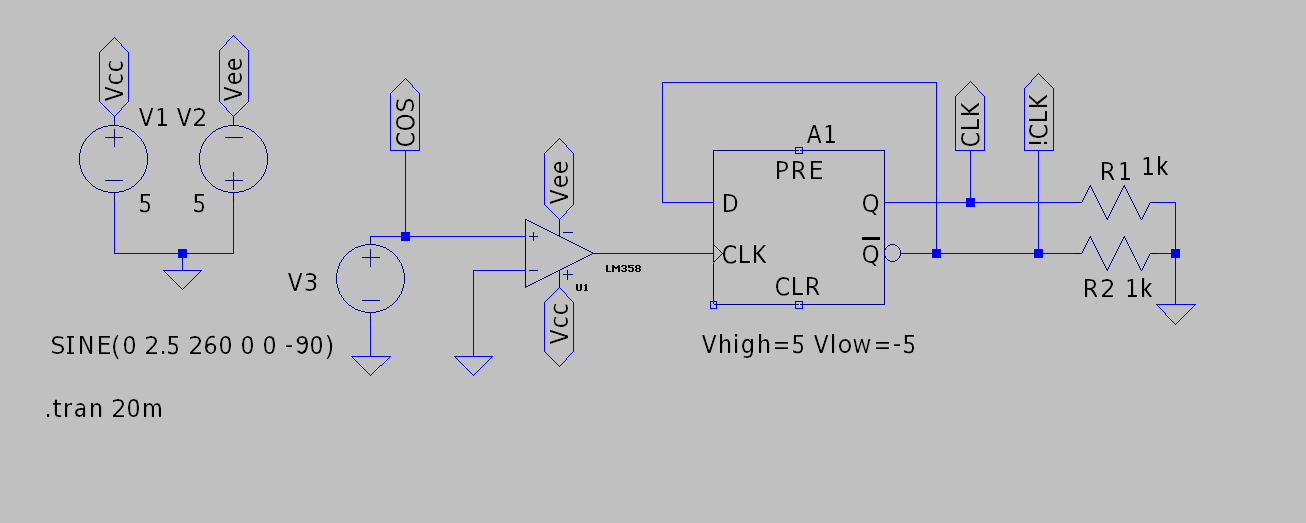
\includegraphics[width=0.65\linewidth]{figs/diseño/3clkCir.png}
    \caption{Circuito con comparador y flip flop simulado en LTSpice}
    \label{clkCir}
\end{figure}

\begin{figure}[H]
    \centering
    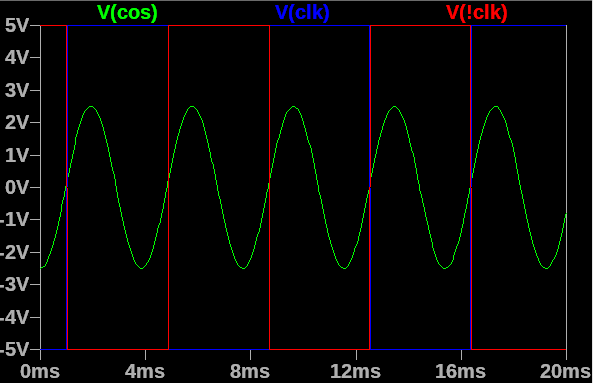
\includegraphics[width=0.65\linewidth]{figs/diseño/3clkSim.png}
    \caption{Entrada y salida del circuito con comparador y flip flop simulado en LTSpice}
    \label{clkSim}
\end{figure}

Como se puede ver en la \figref{clkSim}, la señal cuadrada generada posee un ciclo de trabajo de aproximadamente el 50\% con la mitad de la frecuencia de la señal sinusoidal aplicada a la entrada, así como se obtienen las señales $CLK$ y $\overline{CLK}$ con las amplitudes adecuadas. 
\subsection{Circuito para el control de dibujo de paleta}
Se simularon ambos circuitos correspondientes a esta etapa en LTSpice.
Dichos circuitos han sido diseñados para obedecer las ecuaciones combinacionales \eqref{T} y \eqref{PL}.
Para simular $A_{on}$ y $B_{on}$, se colocaron señales cuadradas con los niveles lógicos del circuito de periodo y ciclo de trabajo cercano, pero diferente, al de la señal $CLK$ y $\overline{CLK}$.
Esto con el propósito de simular varias de las combinaciones binarias entre $A_{on}$, $B_{on}$, $CLK$ y $\overline{CLK}$, para verificar que corresponden al valor correcto de $T$ y $PL$ de acuerdo a las ecuaciones combinacionales que implementan estos circuitos.
Una simulación más rigurosa implicaría analizar toda la tabla de verdad de estos circuitos para asegurar que el circuito corresponde adecuadamente ante cualquier combinación de las señales de entrada.
Sin embargo, debido a cuestiones de tiempo y simplicidad, no se realizará este tipo de simulación. 
Estos circuitos se muestran en la \figref{controlDibujoCir}, mientras que las formas de onda obtenidas de ambos circuitos se muestran en la \figref{controlDibujoSim}.

\begin{figure}[H]
    \centering
    \begin{minipage}{0.6\linewidth}
        \centering
        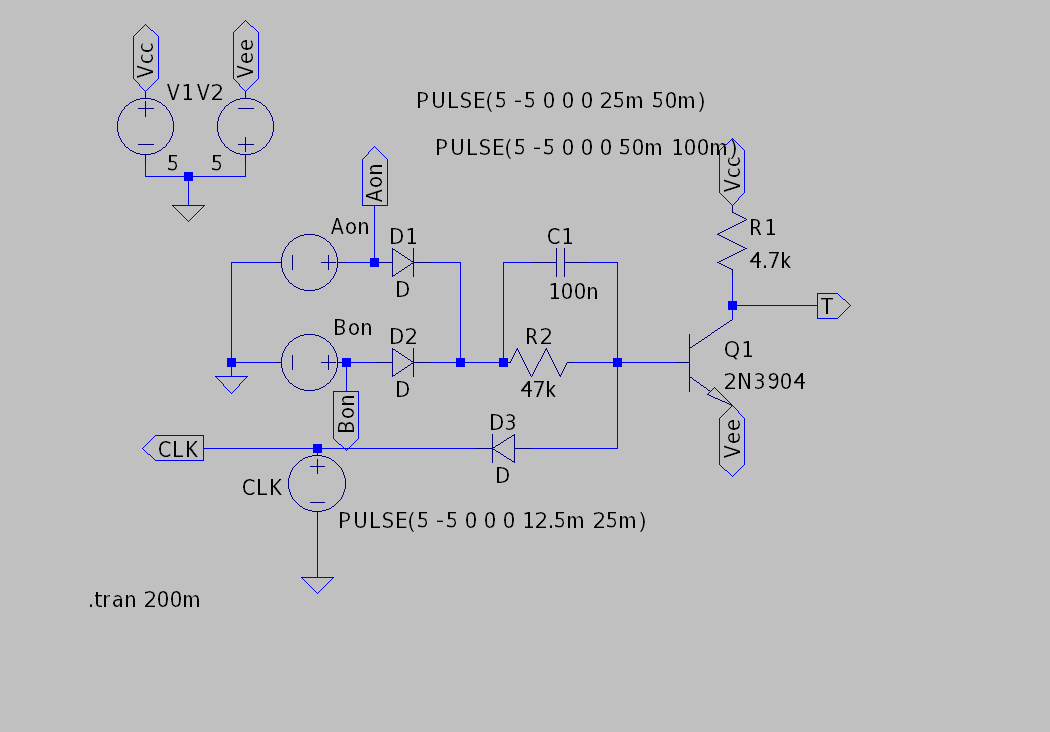
\includegraphics[width=\linewidth]{figs/diseño/4tCir.png}
        \caption*{(a): $T$}
    \end{minipage}\\
    \begin{minipage}{0.6\linewidth}
        \centering
        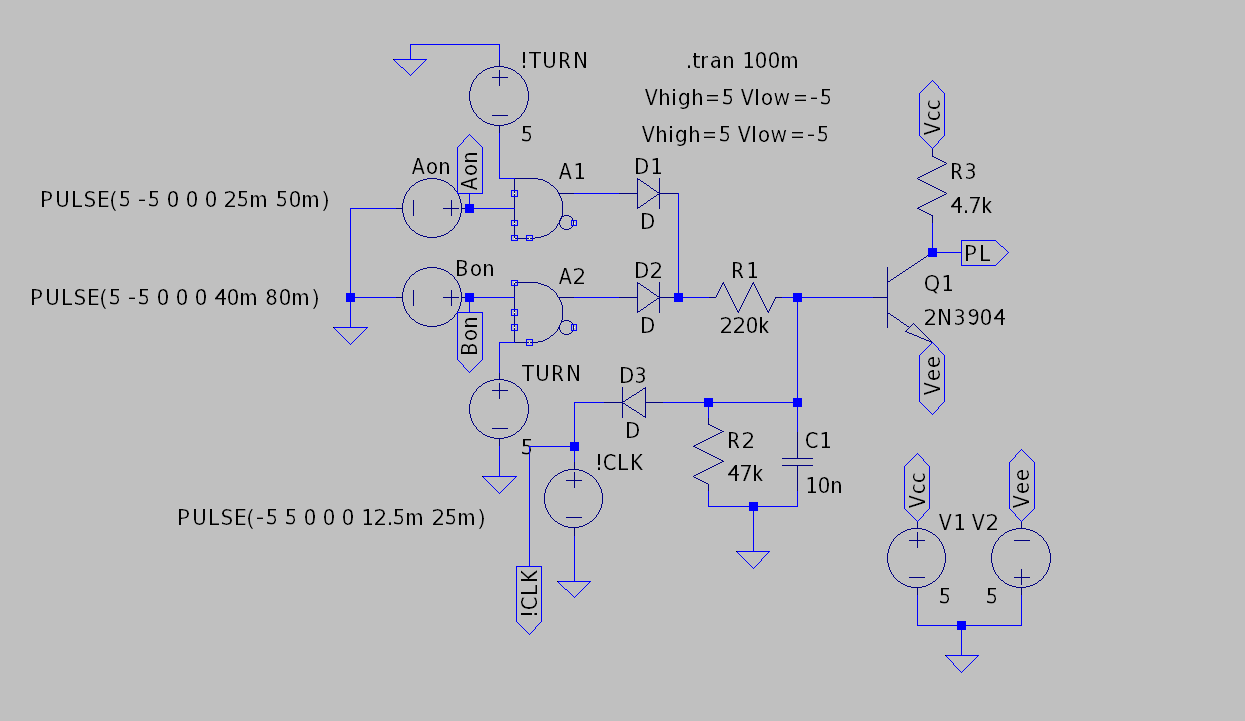
\includegraphics[width=\linewidth]{figs/diseño/4plCir.png}
        \caption*{(b): $PL$}
    \end{minipage}
    \caption{Circuito para el control de dibujo de paleta simulado en LTSpice}
    \label{controlDibujoCir}
\end{figure}

\newpage
\begin{figure}[H]
    \centering
    \begin{minipage}{0.75\linewidth}
        \centering
        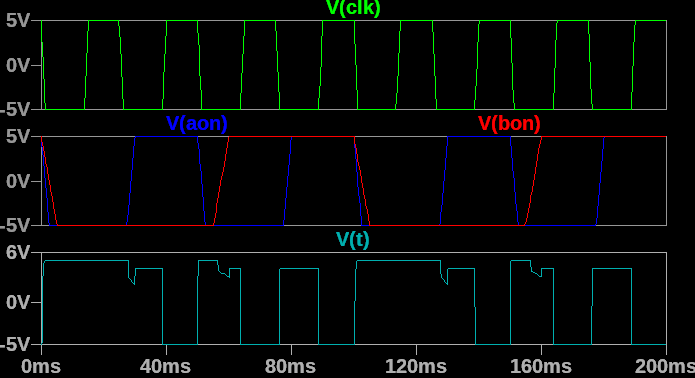
\includegraphics[width=\linewidth]{figs/diseño/4tSim.png}
        \caption*{(a): $T$}
    \end{minipage}\\
    \begin{minipage}{0.75\linewidth}
        \centering
        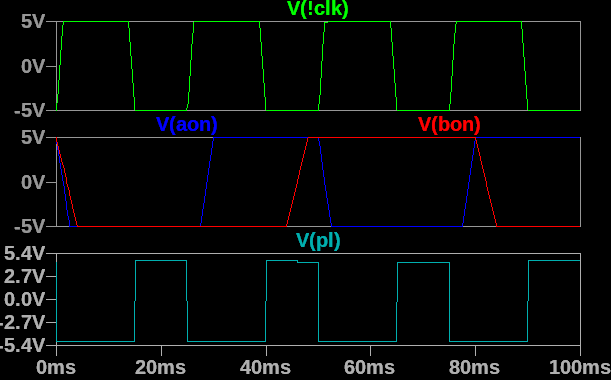
\includegraphics[width=\linewidth]{figs/diseño/4plSim.png}
        \caption*{(b): $PL$}
    \end{minipage}
    \caption{Entrada y salida del circuito con comparador y flip flop simulado en LTSpice}
    \label{controlDibujoSim}
\end{figure}

Se tomaron las combinaciones binarias en las formas de onda que se muestran en la \figref{controlDibujoSim} y se verificaron por medio de las ecuaciones combinacionales \eqref{T} y \eqref{PL}.
Se comprobó que el circuito sí realiza las operaciones lógicas correctamente, así como posee los niveles lógicos adecuados.
Las señales de salida $T$ y $PL$ presentan ciertas distorsiones ante el cambio de señales.
Esto es provocado por la tensión $V_{ce}$ del transistor, la cual no se mantiene constante cuando las señales de entrada cambian, pero se preserva un nivel lógico en la salida. 
Esto puede causar problemas si las señales cambian con alta frecuencia, pero para efectos de este circuito, no resultará ser un gran problema debido a la baja frecuencia producida por el oscilador en cuadratura, del cual se basan el resto de señales periódicas del circuito. 

\subsection{Circuitos multiplexores analógicos 2 a 1, sumadores}
Este circuito no fue simulado en LTSpice debido a que no se encontró un modelo adecuado del componente CD4066 para LTSpice. 
Las salidas de estos circuitos vienen dadas por las ecuaciones \eqref{X} y \eqref{Y}.
\begin{equation}
    ScopeX = \begin{cases}
        \cos(\omega t),&\,T = 0\\
        \cos(\omega t)\frac{P_1}{R_1 + P_1} + BallX\frac{R_1}{R_1 + P_1},&\, T = 1
    \end{cases}\label{X}
\end{equation}  
\begin{equation}
    ScopeY = \begin{cases}
        \sin(\omega t),&\,T = 0\\
        \sin(\omega t)\frac{P_1}{R_2 + P_1} + BallY\frac{R_2}{R_2 + P_1},&\, T = 1\\
    \end{cases}\label{Y}
\end{equation}  

Donde $R_1 = R_2 = \SI{100}{\kohm}$ y $P_1$ se implementa por medio de un potenciómetro de doble gang de valor \SI{10}{\kohm} con el propósito de ajustar simétricamente el tamaño en $X$ y en $Y$ del tamaño de la pelota. 
De esta manera, es posible multiplexar las señales de la pelota y la paleta, siendo la pelota dibujada en los ciclos bajos de $CLK$ y la paleta dibujada en los ciclos en alto de la misma señal, en caso de que sea necesario dibujarla de acuerdo a las señales $A_{on}$ y $B_{on}$.
Adicionalmente, es posible incrementar el tamaño de la pelota desde un punto en la pantalla XY del osciloscopio hasta un tamaño equivalente al círculo del cual se extraen los arcos que corresponden a las paletas. 

\subsection{Circuito con flip flop y circuito RC}
Este circuito fue simulado en LTSpice.
Los potenciómetros se implementarán por medio de un poteciómetro de doble gang de \SI{10}{\kohm} con el propósito de ajustar de forma vectorial la velocidad de la pelota, y no cada componente por aparte con potenciómetros distintos. 
La constante de tiempo mínima y máxima ya ha sido diseñado para estos circuitos, de tal forma que las tensiones de salida del circuito vienen dadas por las ecuaciones \eqref{BallX} y \eqref{BallY}.
\begin{equation}
    BallX = 10\left(1 - e^{\frac{-t}{R_1 + P_1}}\right) -5\label{BallX}
\end{equation}
\begin{equation}
    BallY = 10\left(1 - e^{\frac{-t}{R_2 + P_1}}\right) -5\label{BallY}
\end{equation}

Donde $R_1 = R_2 = \SI{10}{\kohm}$. 
En la \figref{FFRC} se muestra el circuito simulado, y en la \figref{GraficaFFRC} ambas señales de salida de estos circuitos, a los cuales se les aplicó una señal de entrada cuadrada. 

\begin{figure}[H]
    \centering
    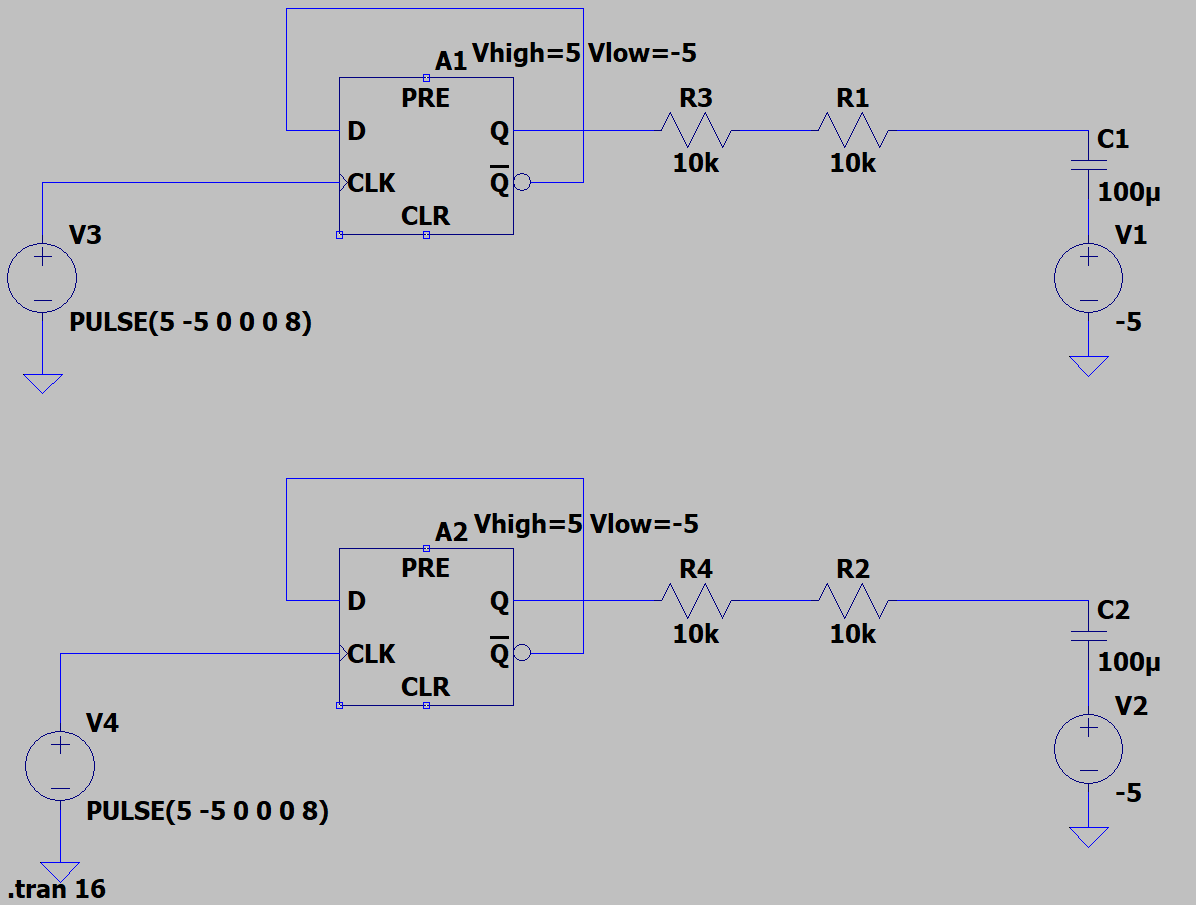
\includegraphics[width=0.8\linewidth]{figs/diseño/6 Circuito con flip flop + circuito RC .png}
    \caption{Circuito con flip flop y circuito RC simulado en LTSpice}
    \label{FFRC}
\end{figure}

\begin{figure}[H]
    \centering
    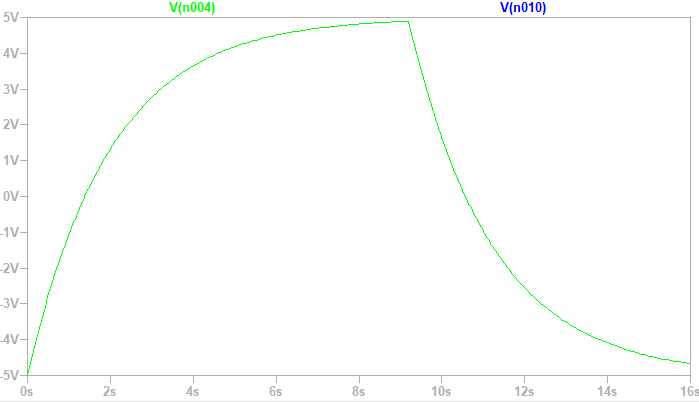
\includegraphics[width=0.8\linewidth]{figs/diseño/6 Circuito con flip flop + circuito RC Graficas de salida BALL X y BALL Y.png}
    \caption{Graficas de salida con las señales $BallX$ y $BallY$ para el circuito con flip flop y circuito RC simulado en LTSpice}
    \label{GraficaFFRC}
\end{figure}

Como se puede ver en la \figref{GraficaFFRC}, inicialmente el capacitor empieza a cargarse debido a que $Q=\SI{5}{V}$, y cuando llega el siguiente flanco positivo de la señal de entrada, la salida del flip flop conmuta, y el capacitor se empieza a descargar.
Debido a que ambos flip flops deben de poseer niveles lógicos de \SI{5}{V} para un 1 lógico y \SI{-5}{V} para un 0 lógico, se tuvo que buscar un modelo de flip flop que admitiera esto.
No se encontraron flip flops D que lograran esto en tiendas de electrónica costarricenses, pero sí se encontraron flip flops tipo JK, CD4027BE, disponible en la página \href{https://www.microjpm.com/products/ad32124/}{MicroJPM}.
Estos flip flops serán alambrados como un flip tipo T con las entradas J y K cortocircuitadas y conectada a \SI{5}{V}, lo cual cumple la misma función que el flip flop D del diseño original.

\subsection{Circuitos comparadores de ventana}

Como ya se había dicho antes, el componente CD4066c no existe en LTspice, por lo tanto, no se logró simular esta etapa.
Esta etapa controla la señal $BOUNCE$, y obedece la ecuación por partes \eqref{bounce}.
\begin{equation}
    BOUNCE = \begin{cases}
        1           & ScopeX = \cos(\omega t)\text{ y } ScopeY=\sin{\omega t}\text{ y }PL = 0\\
        0           & PL = 1
    \end{cases}\label{bounce}
\end{equation}

Es decir, si la posición de la pelota llega a ser la misma que la de las paletas, se levanta la señal $BOUNCE$ para poder determinar si estaba debe rebotar de acuerdo a la circuitería de control correspondiente. 

\subsection{Circuito comparador de ventana para límites horizontales y verticales}
Este circuito fue simulado en LTSpice.
Para ambos comparadores, uno para los límites horizontales y otro para los límites verticales, se utilizarán potenciómetros de doble gang de valor \SI{1}{\kohm} para ajustar las tensiones de umbral de ambos comparadores de forma simétrica, lo cual permite que se ajusten los límites también de forma simétrica. 
El circuito simulado se muestra en la \figref{ComparadorLimites}.
La simulación consistió en aplicar una señal rampa que barriese todas las posibles tensiones que se pueden aplicar a la entrada del comparador, desde \SI{-5}{V} hasta \SI{5}{V}, y analizar el comportamiento de la señal de salida. 
Las señales simuladas se muestran en la \figref{GraficaComparadorLimites}.
Asumiendo que la ventana de tensiones de los comparadores de ventana son $V_x = [V_L^x,\,V_H^x]$ y $V_y = [V_L^y,\,V_H^y]$, los comparadores de ventana por construir responden de acuerdo a las ecuaciones \eqref{yrEq} y \eqref{xrEq}.
\begin{equation}
    XR = \begin{cases}
        1, & BallY\in V_y\\
        0, & BallY\notin V_y
    \end{cases}\label{yrEq}
\end{equation}
\begin{equation}
    YR = \begin{cases}
        1, & BallX\in V_x\\
        0, & BallX\notin V_x
    \end{cases}\label{xrEq}
\end{equation}
Como se puede ver en la \figref{GraficaComparadorLimites}, la tensión de salida del circuito se encuentra en alto únicamente cuando la tensión de entrada se encuentra dentro de ciertas tensiones de umbral.
Para efectos de esta simulación, se simuló por medio de resistencias a que el potenciómetro estuviera en su posición central, de tal manera que las tensiones de umbral vienen dadas por $V_H = \SI{2.5}{V}$ y $V_L = \SI{-2.5}{V}$.
Esto confirma el correcto funcionamiento del comparador de ventana.
Solo es necesario simular uno de los comparadores de ventana, ya que ambos circuitos son una copia uno del otro, con diferentes tensiones de entrada.

\begin{figure}[H]
    \centering
    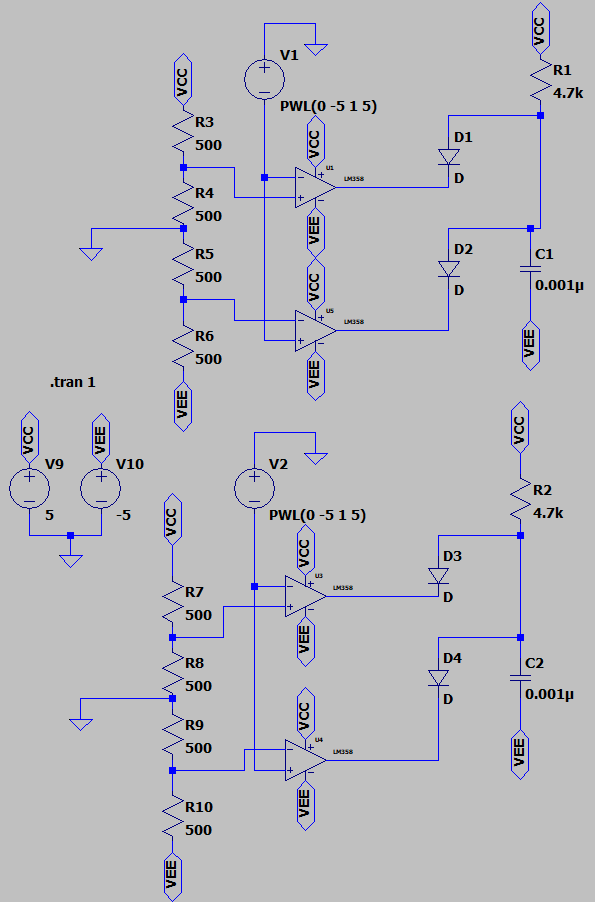
\includegraphics[width=0.7\linewidth]{figs/diseño/8 Circuitos comparadores de ventana para los limites .png}
    \caption{Circuitos comparadores de ventana para los límites horizontales y verticales de la pantalla
del juego simulados en LTSpce}
    \label{ComparadorLimites}
\end{figure}

\begin{figure}[H]
    \centering
    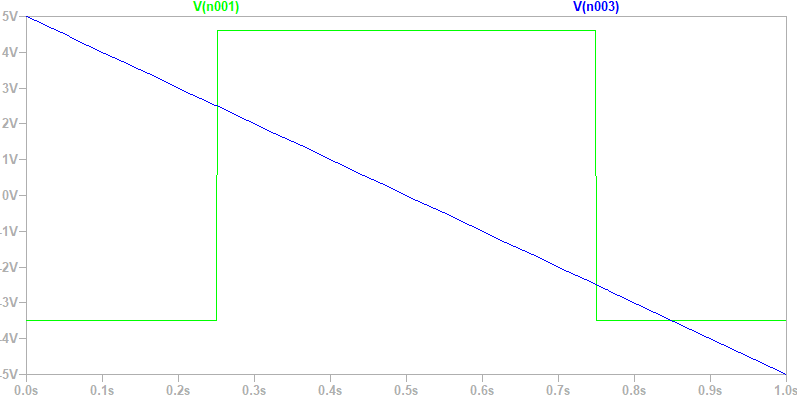
\includegraphics[width=0.8\linewidth]{figs/diseño/8 Circuitos comparadores de ventana para los limites, Graficas entrada y salida.png}
    \caption{Entrada y salida del circuito comparador de ventana para los límites horizontales simulado en LTSpice}
    \label{GraficaComparadorLimites}
\end{figure}


\subsection{Circuito para el control de dirección de la pelota}
Este circuito permite determinar las señales $XREV$ y $YREV$, cuyo flanco positivo invierte la dirección de desplazamiento de la pelota.
Esto sucede si se detecta un rebote a partir de la señal $BOUNCE$ y se activan las señales $XR$ o $YR$.
Este circuito cuenta con un botón para posicionar la pelota en la posición central de la pantalla del osciloscopio.
Debido a que no se encontró una forma de simular el pulsado de un botón en LTSpice en un momento en particular, no se simuló esta parte. 
El circuito simulado se muestra en la \figref{DirecPelota}.
Se simuló el circuito con la señal $BOUNCE$ con un valor constante, y una onda cuadrada en $XR$ Y $YR$.
Las señales de entrada y salida del circuito se muestran en la \figref{GraficaDirecPelota}.
Como se puede ver en la gráfica, la señal $XREV$ reacciona de la misma manera que la entrada aplicada al circuito, gracias a que la compuerta AND se convierte transparente una vez la señal $BOUNCE$ está en alto, mostrando el correcto funcionamiento del circuito. 
Las señales de salida del circuito obedecen las ecuaciones \eqref{XREV} y \eqref{YREV}.
\begin{equation}
    XREV = \begin{cases}
        1, & XR \cdot BOUNCE + Pulsador = 1\\
        0, & \text{en caso contrario}
    \end{cases}\label{XREV}
\end{equation}
\begin{equation}
    YREV = \begin{cases}
        1, & YR \cdot BOUNCE + Pulsador = 1\\
        0, & \text{en caso contrario}
    \end{cases}\label{YREV}
\end{equation}
\begin{figure}[H]
    \centering
    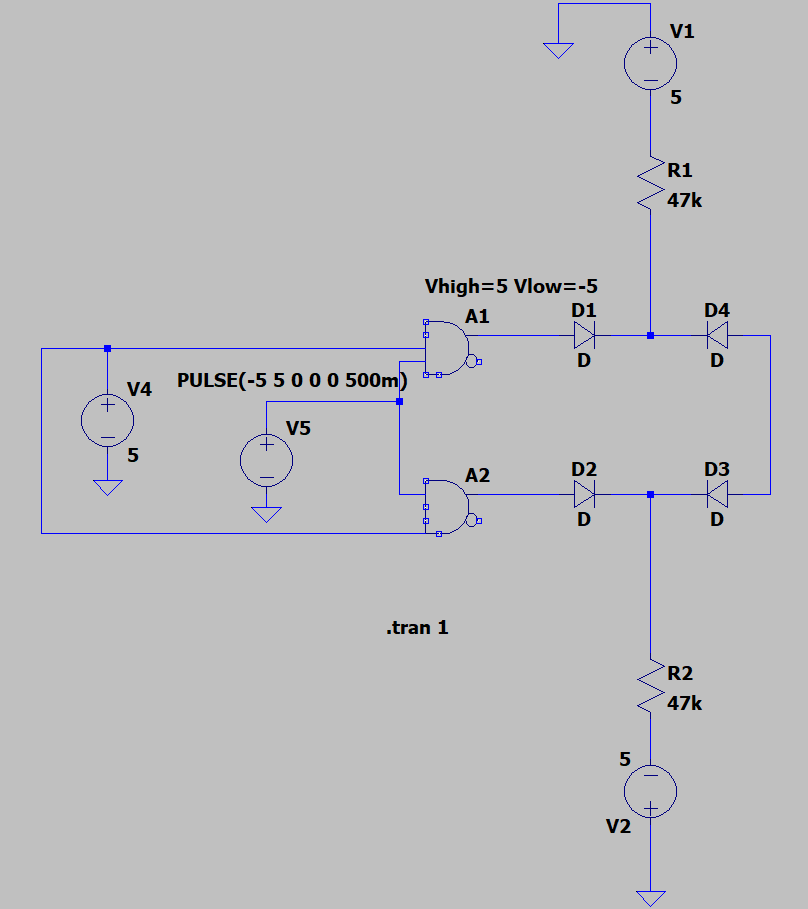
\includegraphics[width=0.7\linewidth]{figs/diseño/9 Circuito para el control de direccion de la pelota.png}
    \caption{Circuito para el control de direccion de la pelota }
    \label{DirecPelota}
\end{figure}

\begin{figure}[H]
    \centering
    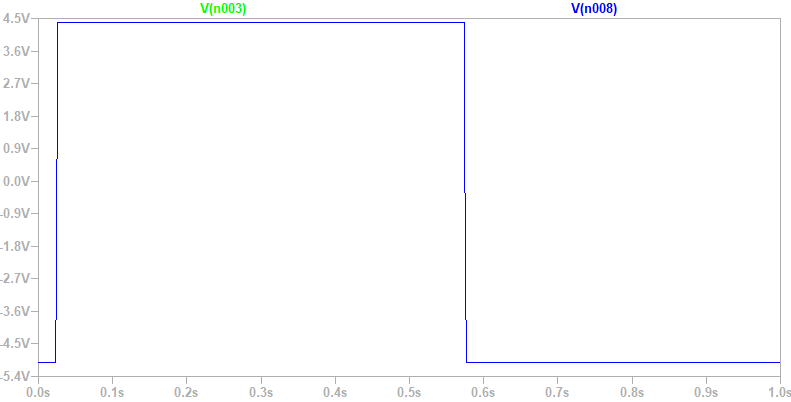
\includegraphics[width=0.8\linewidth]{figs/diseño/9 Circuito para el control de direccion de la pelota Graficas de XREV Y YREV.png}
    \caption{Circuito para el control de direccion de la pelota Graficas de XREV Y YREV}
    \label{GraficaDirecPelota}
\end{figure}
\newpage

\subsection{Circuito para el control de turnos y LEDs indicadores}
Este circuito fue simulado en LTSpice, aplicando una señal cuadrada a la entrada.
Se verificó que las señales $TURN$ y $\overline{TURN}$ tuvieran el comportamiento adecuada, siendo cada una de estas una el inverso de la otra.
En la \figref{ControlTurnosLed} se muestra el circuito simulado, y habiendo aplicado una señal cuadrada a la entrada del circuito, se muestra en \figref{GraficaControlTurnosLed} las señales de salida del circuito.
Como se puede observar, se obtienen las salidas complementarias, mostrando el correcto funcionamiento del circuito. 

\begin{figure}[H]
    \centering
    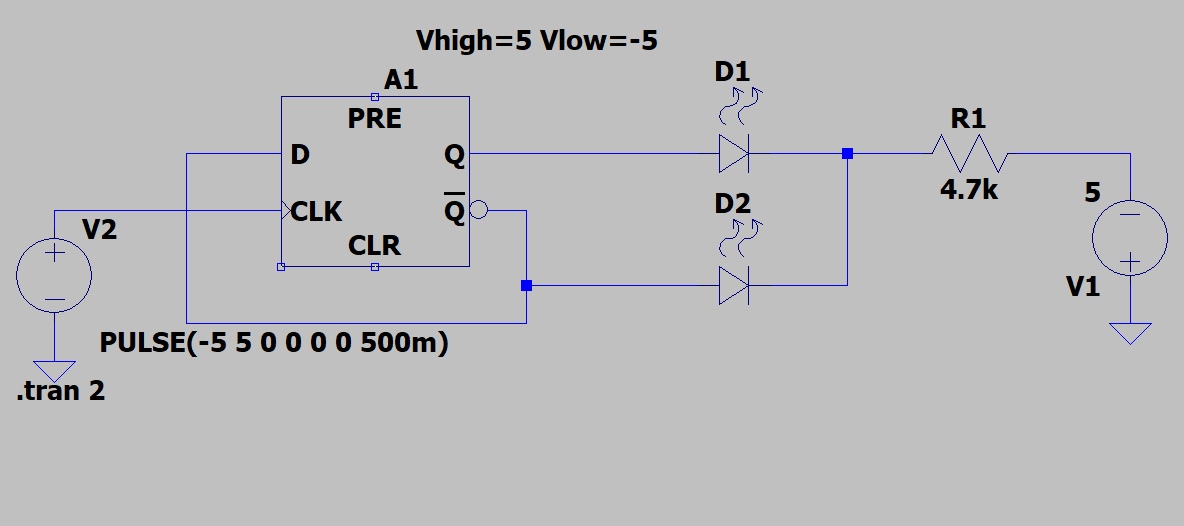
\includegraphics[width=0.8\linewidth]{figs/diseño/10 Circuito para el control de turnos y LEDs indicadores .png}
    \caption{Circuito para el control de turnos y LEDs indicadores}
    \label{ControlTurnosLed}
\end{figure}

\begin{figure}[H]
    \centering
    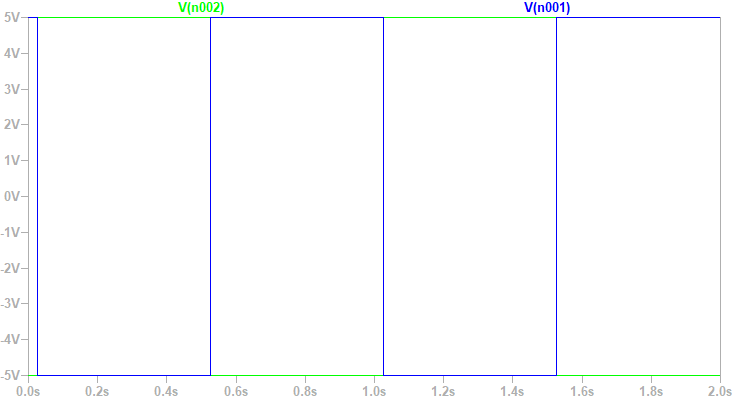
\includegraphics[width=0.8\linewidth]{figs/diseño/10 Circuito para el control de turnos y LEDs indicadores, Grafica de TURN yTURN negado.png}
    \caption{Circuito para el control de turnos y LEDs indicadores, Grafica de TURN y TURN negado.}
    \label{GraficaControlTurnosLed}
\end{figure}


\subsection{Circuito para efectos de sonido}

Para esta etapa se decidió qué debido a que este proyecto tiene muchas etapas y esta etapa no agrega funcionalidad al circuito. Se decidió quitarla del experimento, y si existiera tiempo adicional después de que todas las etapas estén construidas, se reconsiderará construirla.